\section{Interferenz}

\subsection{Einleitung}
Bei diesem Experiment soll die Wellenlänge $\lambda$ eines roten und eines grünen Laserpointers bestimmt werden.
Für die Bestimmung wird der Wellencharakter von Licht ausgenutzt, Licht wird nämlich, wenn es auf einen Doppelspalt trifft gebeugt und es entsteht ein Interferenzmuster(Abbildung 1).\\
Zum erzeugen so eines Interferenzmuster wird auf einer optischen Schiene zuerst der Laserpointer befestigt. Dann wird der Doppelspalt so montiert, dass der Lichtstrahl genau darauf trifft, 
ans Ende wird dann noch eine Schirm aufgestellt, auf welchem das Interferenzmuster abgebildet wird. Der Abstand zwischen Schirm und Doppelspalt beträgt $d$, diese Größe ist später
zur berechnung der Wellenlänge wichtig. \\
Auf dem Schirm sind die Interferenzmaxima -und minima zu erkennen(Abbildung 1). Zur Berechnung der Wellenlänge braucht man jetzt noch den Abstand $x$ einer bestimmten Zahl an solchen Maxima und die Anzahl
der Maxima über die gemessen wird, wobei man mit 0 anfängt zu zählen. 
\begin{figure}[H]
    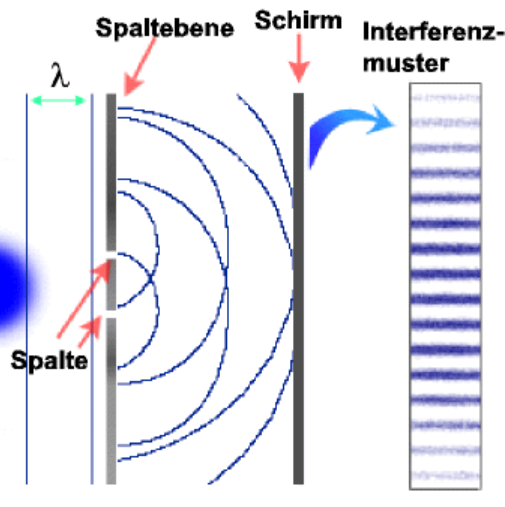
\includegraphics[scale=0.5]{C:/Users/josefk/Desktop/Spektroskopie/src/img/interfernez.PNG}
    \caption{Interferenzmuster welches von Licht erzeugt wird, wenn es auf einen Doppelspalt trifft.}
\end{figure}

\subsection{Berechnung}
\begin{itemize}
    \item Bestimmung von $\alpha$
    \begin{align*}
        &\tan \alpha = \frac{x} {d} \Rightarrow \alpha = \arctan \frac{x} {d}\\
        &\arctan \frac{0.94}{50.7} = 1.06
    \end{align*}         
        \begin{tabular}{ll}
        x... Abstand zwischen gemessenen Maxima & d... Abstand vom Schirm zum Doppelspalt \\
        $\alpha$... Winkel &
        \end{tabular}  
    \item 
\end{itemize}

\begin{figure}[H]
    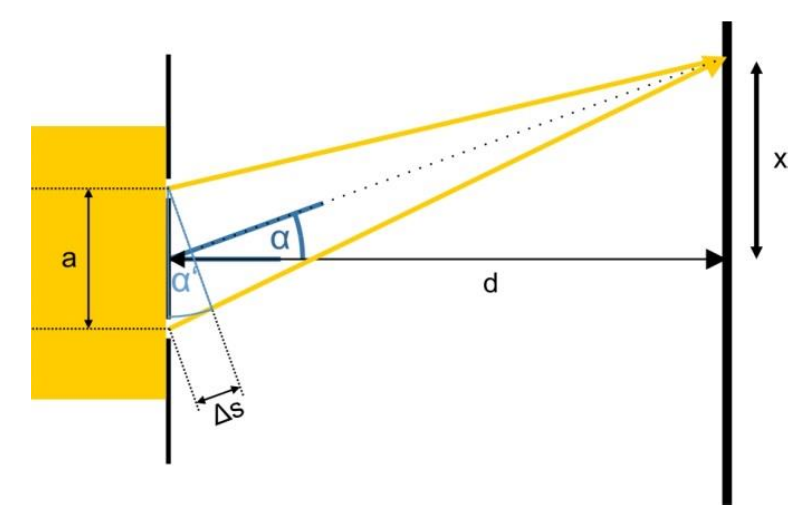
\includegraphics[scale=0.5]{C:/Users/josefk/Desktop/Spektroskopie/src/img/berechnung.PNG}
    \caption{Doppelspalt. Paralleles Licht trifft auf einen
    Doppelspalt mit dem Abstand $a$ zwischen den beiden Einzelspalten.
    Auf einem Schirm im Abstand $d$ kann eine winkelabhängige
    Intensitätsverteilung beobachtet werden. Ein Maximum ist erkennbar
    wenn der Gangunterschied $\Delta s$ ein Vielfaches der Wellenlänge $\lambda$ ist.}
\end{figure}
